\documentclass[12pt]{article}
\usepackage{tikz}
\usepackage{amsmath}
\usepackage[a4paper, portrait, margin=1cm]{geometry}
% \usepackage{multicol}
\usepackage{fancyhdr}
\def \HeadingAnswers {\section*{\Large Name: \underline{\hspace{8cm}} \hfill Date: \underline{\hspace{3cm}}} \vspace{-3mm}
{Levers: Answers} \vspace{1pt}\hrule}

% raise footer with page number; no header
\fancypagestyle{myfancypagestyle}{
  \fancyhf{}% clear all header and footer fields
  \renewcommand{\headrulewidth}{0pt} % no rule under header
  \fancyfoot[C] {\thepage} \setlength{\footskip}{6pt} % raise page number 6pt
}
\pagestyle{myfancypagestyle}  % apply myfancypagestyle

\newcounter{minipagecount}

\begin{document}
\HeadingAnswers
\vspace{8mm}

\refstepcounter{minipagecount}
\noindent\textbf{\theminipagecount.}\quad

\begin{minipage}{0.5\textwidth}
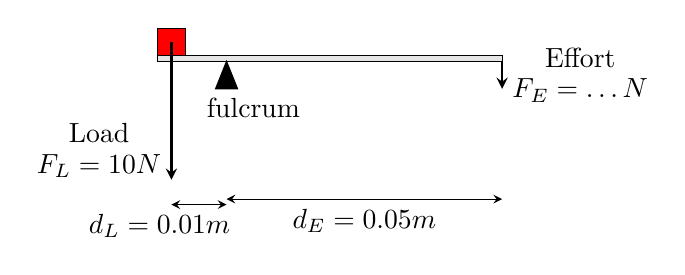
\begin{tikzpicture}[scale=0.7,>=stealth]
% First class lever
% rod
\draw[fill=gray!20] (-0.25,0) rectangle (6,0.1);
%fulcrum
\draw[fill=black] (0.8,-0.5) -- (1.2,-0.5) node[below,xshift=2mm] {fulcrum} -- (1.0,0) -- cycle;
%load
\draw[fill=red] (-0.25,0.1) rectangle (0.25,0.6);
\draw[->,thick] (0.0,0.35) -- (0.0,-2.15) node[midway,left,yshift=-0.5cm,align=center] {Load \\\\[-3ex] $F_L = 10N$};
%effort
\draw[->,thick] (6,0.0) -- (6,-0.5) node[midway,right,align=center] {Effort \\\\[-3ex] $F_E = \dots N$};

% Distance markers
\draw[<->] (1,-2.5) -- (6,-2.5) node[midway,below,align=center] {$d_E = 0.05m$};
\draw[<->] (0,-2.6) -- (1.0,-2.6) node[midway,below,xshift=-0.5cm,align=left] {$d_L = 0.01m$};


\end{tikzpicture}
\end{minipage}%
\hfill
\begin{minipage}{0.5\textwidth}
\begin{flalign*}
&& F_E \times d_E &= F_L \times d_L && \\
&& F_E &= \frac{F_L \times d_L}{d_E} && \\
&& F_E &= \frac{10 \times 0.01}{0.05} && \\
&& F_E &= 2N &&
\end{flalign*}
\end{minipage}



\end{document}
